% Options for packages loaded elsewhere
\PassOptionsToPackage{unicode}{hyperref}
\PassOptionsToPackage{hyphens}{url}
%
\documentclass[
]{article}
\usepackage{lmodern}
\usepackage{amssymb,amsmath}
\usepackage{ifxetex,ifluatex}
\ifnum 0\ifxetex 1\fi\ifluatex 1\fi=0 % if pdftex
  \usepackage[T1]{fontenc}
  \usepackage[utf8]{inputenc}
  \usepackage{textcomp} % provide euro and other symbols
\else % if luatex or xetex
  \usepackage{unicode-math}
  \defaultfontfeatures{Scale=MatchLowercase}
  \defaultfontfeatures[\rmfamily]{Ligatures=TeX,Scale=1}
\fi
% Use upquote if available, for straight quotes in verbatim environments
\IfFileExists{upquote.sty}{\usepackage{upquote}}{}
\IfFileExists{microtype.sty}{% use microtype if available
  \usepackage[]{microtype}
  \UseMicrotypeSet[protrusion]{basicmath} % disable protrusion for tt fonts
}{}
\makeatletter
\@ifundefined{KOMAClassName}{% if non-KOMA class
  \IfFileExists{parskip.sty}{%
    \usepackage{parskip}
  }{% else
    \setlength{\parindent}{0pt}
    \setlength{\parskip}{6pt plus 2pt minus 1pt}}
}{% if KOMA class
  \KOMAoptions{parskip=half}}
\makeatother
\usepackage{xcolor}
\IfFileExists{xurl.sty}{\usepackage{xurl}}{} % add URL line breaks if available
\IfFileExists{bookmark.sty}{\usepackage{bookmark}}{\usepackage{hyperref}}
\hypersetup{
  pdftitle={Ćwiczenie 1},
  pdfauthor={Karol Hamielec},
  hidelinks,
  pdfcreator={LaTeX via pandoc}}
\urlstyle{same} % disable monospaced font for URLs
\usepackage[margin=1in]{geometry}
\usepackage{graphicx}
\makeatletter
\def\maxwidth{\ifdim\Gin@nat@width>\linewidth\linewidth\else\Gin@nat@width\fi}
\def\maxheight{\ifdim\Gin@nat@height>\textheight\textheight\else\Gin@nat@height\fi}
\makeatother
% Scale images if necessary, so that they will not overflow the page
% margins by default, and it is still possible to overwrite the defaults
% using explicit options in \includegraphics[width, height, ...]{}
\setkeys{Gin}{width=\maxwidth,height=\maxheight,keepaspectratio}
% Set default figure placement to htbp
\makeatletter
\def\fps@figure{htbp}
\makeatother
\setlength{\emergencystretch}{3em} % prevent overfull lines
\providecommand{\tightlist}{%
  \setlength{\itemsep}{0pt}\setlength{\parskip}{0pt}}
\setcounter{secnumdepth}{-\maxdimen} % remove section numbering

\title{Ćwiczenie 1}
\author{Karol Hamielec}
\date{3/10/2020}

\begin{document}
\maketitle

\(\vspace{1.5cm}\) \#\# zad1

\#\#\#Wykorzystując bazę̨ danych yelp dataset wykonaj zapytanie i komendy
MongoDB, aby uzyskać́ następujące rezultaty:

\begin{itemize}
\item ~
  \hypertarget{a-zwruxf3ux107-bez-powtuxf3rzeux144-wszystkie-nazwy-miast-w-ktorych-znajduja-sie-firmy-business.-wynik-posortuj-na-podstawie-nazwy-miasta-alfabetycznie.}{%
  \paragraph{a) Zwróć́ bez powtórzeń́ wszystkie nazwy miast w których
  znajdują się firmy (business). Wynik posortuj na podstawie nazwy
  miasta
  alfabetycznie.}\label{a-zwruxf3ux107-bez-powtuxf3rzeux144-wszystkie-nazwy-miast-w-ktorych-znajduja-sie-firmy-business.-wynik-posortuj-na-podstawie-nazwy-miasta-alfabetycznie.}}

  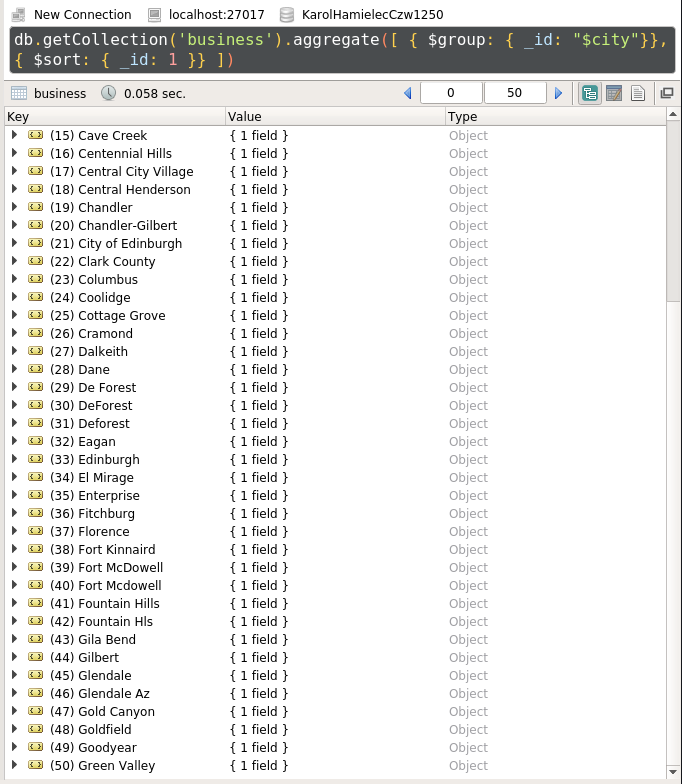
\includegraphics{./images/0.jpg}~
  \texttt{db.getCollection(\textquotesingle{}business\textquotesingle{}).find(\{open:\ true\},\{\ name:\ 1,\ \ \ \ \ \ full\_address:\ 1,\ \ \ \ \ \ stars:\ 1\})}
\item ~
  \hypertarget{b-zwruxf3ux107-liczbux119-wszystkich-recenzji-ktuxf3re-pojawiux142y-siux119-po-2011-roku-wux142acznie.}{%
  \paragraph{b) Zwróć́ liczbę̨ wszystkich recenzji, które pojawiły się̨ po
  2011 roku
  (włącznie).}\label{b-zwruxf3ux107-liczbux119-wszystkich-recenzji-ktuxf3re-pojawiux142y-siux119-po-2011-roku-wux142acznie.}}

  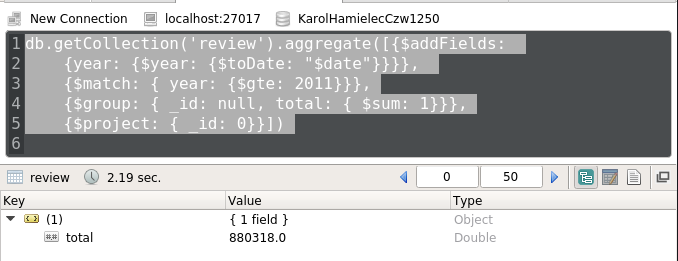
\includegraphics{./images/1.jpg}~
\item ~
  \hypertarget{c-zwruxf3ux107-dane-wszystkich-zamkniux119tych-open-firm-business-z-pol-nazwa-adres-gwiazdki-stars.}{%
  \paragraph{c) Zwróć́ dane wszystkich zamkniętych (open) firm (business)
  z pól: nazwa, adres, gwiazdki
  (stars).}\label{c-zwruxf3ux107-dane-wszystkich-zamkniux119tych-open-firm-business-z-pol-nazwa-adres-gwiazdki-stars.}}

  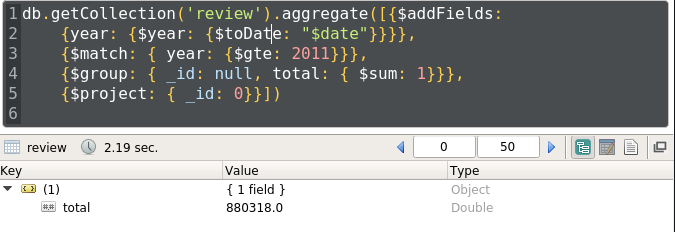
\includegraphics{./images/2.jpg}~
\item ~
  \hypertarget{d-zwruxf3ux107-dane-wszystkich-uux17cytkownikuxf3w-user-ktuxf3rzy-nie-uzyskali-ani-jednego-pozytywnego-gux142osu-z-kategorii-funny-lub-useful-wynik-posortuj-alfabetycznie-wedux142ug-imienia-uux17cytkownika.}{%
  \paragraph{d) Zwróć́ dane wszystkich użytkowników (user), którzy nie
  uzyskali ani jednego pozytywnego głosu z kategorii (funny lub useful),
  wynik posortuj alfabetycznie według imienia
  użytkownika.}\label{d-zwruxf3ux107-dane-wszystkich-uux17cytkownikuxf3w-user-ktuxf3rzy-nie-uzyskali-ani-jednego-pozytywnego-gux142osu-z-kategorii-funny-lub-useful-wynik-posortuj-alfabetycznie-wedux142ug-imienia-uux17cytkownika.}}

\begin{verbatim}
db.getCollection('user').find({ $or: 
    [ {"votes.funny": 0}, {"votes.useful": 0}]}).sort({ name: 1})
\end{verbatim}
\item ~
  \hypertarget{e-okreux15bl-ile-kaux17cde-przedsiux119biorstwo-otrzymaux142o-wskazoweknapiwkow-tip-w-2012.-wynik-posortuj-alfabetycznie-wedux142ug-liczby-tip.}{%
  \paragraph{e) Określ, ile każde przedsiębiorstwo otrzymało
  wskazówek/napiwków (tip) w 2012. Wynik posortuj alfabetycznie według
  liczby
  (tip).}\label{e-okreux15bl-ile-kaux17cde-przedsiux119biorstwo-otrzymaux142o-wskazoweknapiwkow-tip-w-2012.-wynik-posortuj-alfabetycznie-wedux142ug-liczby-tip.}}

\begin{verbatim}
db.getCollection('tip').aggregate([
    { $match: { date: {$regex: "^2012.*"}}},
    { $group: { _id: "$business_id" , count: {$sum: 1}}},
    { $sort: { count: 1 }}
])
\end{verbatim}
\item ~
  \hypertarget{f-wyznacz-jaka-ux15brednia-ocen-stars-uzyskaux142a-kaux17cda-firma-business-na-podstawie-wszystkich-recenzji.-wynik-ogranicz-do-recenzji-ktuxf3re-uzyskaux142y-min-4.0-gwiazdki.}{%
  \paragraph{f) Wyznacz, jaką średnia ocen (stars) uzyskała każda firma
  (business) na podstawie wszystkich recenzji. Wynik ogranicz do
  recenzji, które uzyskały min 4.0
  gwiazdki.}\label{f-wyznacz-jaka-ux15brednia-ocen-stars-uzyskaux142a-kaux17cda-firma-business-na-podstawie-wszystkich-recenzji.-wynik-ogranicz-do-recenzji-ktuxf3re-uzyskaux142y-min-4.0-gwiazdki.}}

\begin{verbatim}
db.getCollection('review').aggregate([
    {$group: { _id: "$business_id", avg: {$avg: "$stars" }}},
    {$match: { avg: { $gt: 4.0}}}
])
\end{verbatim}
\item ~
  \hypertarget{g-usuux144-wszystkie-firmy-business-ktuxf3re-posiadajux105-ocenux119-stars-ruxf3wna-2.0.}{%
  \paragraph{g) Usuń́ wszystkie firmy (business), które posiadają̨ ocenę̨
  (stars) równą
  2.0.}\label{g-usuux144-wszystkie-firmy-business-ktuxf3re-posiadajux105-ocenux119-stars-ruxf3wna-2.0.}}
\end{itemize}

\end{document}
